\chapter{Introduction}
\section{High frequency trading system}
\subsection{Evolution of high-frequency trading}
Over the last few decades, information technology, including computing speed and memory volume, has made a great development. According to this trend, a new class of trading system, which is called high-frequency trading (HFT), has appeared to today's financial markets. Generally speaking,  HFT represents a program trading platform that uses powerful computers to transact a great number of orders at very fast speeds. It becomes more and more attractive  because of some key factors:\\
\begin{itemize}
\item \textbf{Narrowing Spreads}. In 2001, the unit of quoting prices in U.S. Stock exchanges changed from fractions to decimals. So the minimum spread between the bid and ask prices decreased from 1/6th of a dollar (6.25 cents) to one cent. The change of price unit provides traders better alternatives to seeking spread arbitrages, which results in a strong boost in an algorithmic trading system.  \\
\item \textbf{Regulation changes}. In 2005, the Securities and Exchange Commission(SEC) passed the Regulation National Market System(Reg.NMS), which improved transparency and competition among different financial markets. Besides, this regulation also required trade orders to be posted nationally instead of at individual exchanges. So traders can be beneficial of profit from small price difference of one security among different exchanges. \\
\end{itemize}

High-frequency trading is an extension case of algorithmic trading, which turns over small positions of security very frequently. The U.S. Securities and Exchanges Commission conclude specific characteristics of HFT:\\

\begin{itemize}
\item Submit some orders and cancel them soon after the submission.
\item Maintain very few or no overnight positions. 
\item Maintain a very high turn over rate of a very small positions of a specific security or evena pool of securities. Meanwhile the holding period for each position is also very short.
\item Utilize complicated and high-performance computing program to generate, execute or cancel orders.
\item Utilize individual data from exchanges and servers that belong to co-location provider that minimize network or other types of latencies. 
\end{itemize}

According to recent survey(\cite{hft_future}), high-frequency trading has taken a great number of share in U.S. and European equity trading volume. As shown in figure \ref{fig.1}, in U.S., the percentage of HFT in equity turnover by volume maintained growth trend overall from year the 2005 to 2010. For example, in 2010, HFT occupied 56\% by volume of the entire equity turnover, increased from 21 \% in 2005. 

\begin{figure}[hbtp]
  \begin{center}
    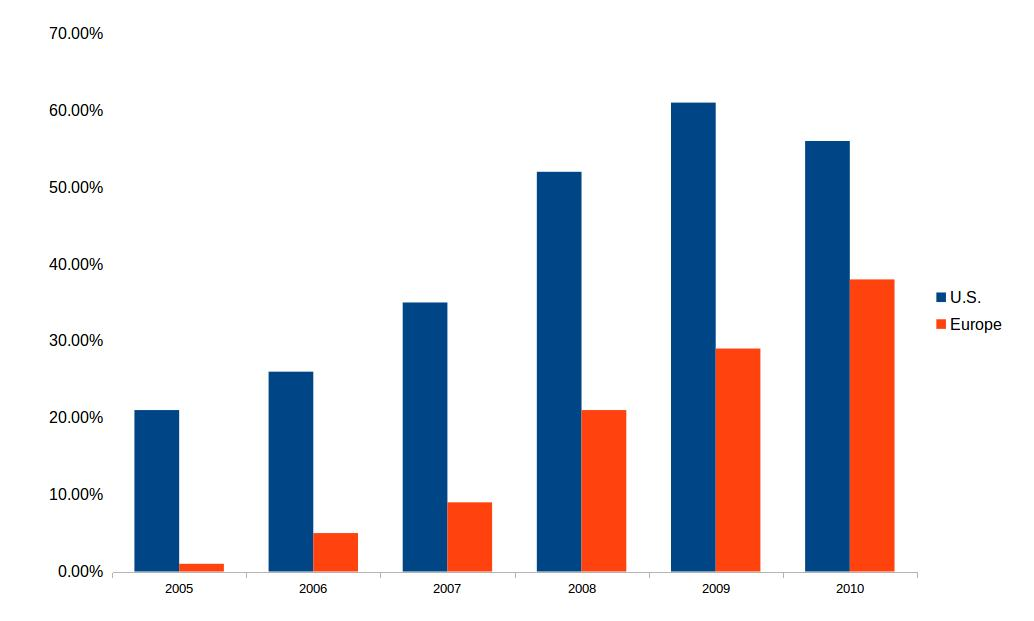
\includegraphics[width=6.5in,height=3.5in]{figures/hft_percentage.jpg}
  \end{center}
\caption{High frequency trading as a \% of equity turnover by volume, U.S. and by value, Europe 2005-2010} \label{fig.1}
\end{figure}

A similar situation happened in Europe. HFT only accounted for 1\% of equity turnover by value in 2005. The percentage surged to 38 \% in 2010, increased from 29 \% just a year ago.
\subsection{High frequency trading strategies}
Generally speaking, there are two main high-frequency trading strategies: passive and aggressive trading strategies. Passive strategies use limit orders which let the brokerage to buy or sell the stocks at a specified level price, while aggressive strategies utilize market orders to buy or sell the stocks immediately. In the following, we give the description of main types of these two trading strategies. 

For passive HFT strategies, the first widely used method is passive market making. This method allows the market maker to purchase a company's securities and, at the same time, the market maker is also acted as an underwriter of the 
securities in a secondary public offering. Since the market maker can place bids of a security before its publication, the real buyers would have to place their buy orders higher than the market maker's bid price. Therefore the market maker can  benefit from this higher opening. The second method for passive strategies is arbitrage trading. As described by its name, this method makes a profit by the price difference of the same or related securities. A simple example is as follows: the stock of one company that we called X is trading at \$10 on the New York Stock Exchange(NYSE), while at the same moment it is trading at the price of \$10.05 on the London Stock Exchange(LSE).  Given that a trader can trade the stock on both markets with no time lag, he can buy one specific security on the NYSE and sell the same shares on the LSE just after buying. Obviously, a profit of 5 cents without risk can be earned by him. Those arbitrage opportunity will persist until the specialists on the NYSE or LSE adjust their price to eliminate the price difference.

The main type of aggressive HFT strategies consists of the following two types:
Momentum ignition and order anticipate. The former one is a strategy that a proprietary trading firm buy or sell volumes of orders that will cause the price of underlying security significantly going up or down shortly. Such quick submission and cancellation of many orders of a stock will trigger other traders' algorithm to buy or sell the same stock more aggressively. After the trend of price movement is made in the market, the momentum maker will benefit from selling the stock at a higher price or buying the stock at a lower price. However it is very difficult to distinguish between momentum ignition and $\textit{spoof}$, which was defined as illegal according to Dodd-Frank Act.  For the order anticipate method, it can be described as a liquidity detection trading which confirms the existence of large institutional buys or sellers in the marketplace and then trades ahead of these buyers or sellers in anticipation that their large orders will move market prices( Securities and Exchange Commission,2014,p.8). The line between this method and another illegal action called \textit{front-running} can be nuanced. The \textit{front-running} is the unethical practice that a stockbroker trades securities in his personal account based on the knowledge of advance knowledge of pending orders from its customers. 

\section{Limit order book dynamics}
According to the above section, we know that under the aggressive strategies situation, it is very likely that the strategy will be deemed as illegal. Therefore choosing passive strategies in high-frequency trading is a good idea. Since most transactions in the passive trading strategies are buying and selling the securities at a particular price, limit order books play an indispensable role in this strategy.  
Actually, in today's financial market, more than half of stock exchanges now use a limit order book(LOB) mechanism to facilitate trade(\cite{rosu2009dynamic}).  Some exchanges, such as Helsinki, Hong Kong, Shenzhen, Swiss, Tokyo, Toronto, and
Vancouver Stock Exchanges, now use pure LOBs(\cite{luckock2001statistical}). Some exchanges use hybrid of hybrid LOBs, which include  the New York Stock Ex-change (NYSE), NASDAQ, and the London Stock Exchange
(LSE) \citep{cont2010stochastic}. 

As described above, we can see that LOBs play an major role in financial trading architectures, it is beneficial for both scholars and practitioners to understand dynamics of LOB. The advantages of capturing dynamics of LOBs include: finding optimal opportunity to execute orders\citep{obizhaeva2013optimal}; improving the performance of electronic trading algorithms\citep{engle2006measuring}; Obtaining a better understanding of micro market structure for Practitioners\citep{harris2003trading}; Getting a clearer insight into market volatility\citep{kirilenko2015flash}.

In this thesis, we first introduce basic definitions of LOBs, including math definition of the bid-ask spread, mid price, bid and ask side depth, spread crossing opportunities and so on. Then we use statistical and data driven methods,especially in the area of machine learning architectures, to model the future arbitrage opportunities of LOBs. We focus on ensemble machine learning algorithms to build our prediction models. As far as we know, there is no evidence shows that these methods were used in LOBs research area. The introduction of ensemble machine learning algorithms will be given in the following section of this chapter and details can be found in chapter \ref{ch:ensemble}.  


\section{Ensemble method for classifiers}

In spite of a great amount of research on limit order books, there is only a few literature which utilizes machine learning methods for capturing the limit order books. Furthermore, based on our knowledge, there is little evidence that ensemble methods were allied to this topic. In our research, we try to use AdaBoost(Adaptive Boosting) method, which was deemed as the best classifier off the shelf\citep{kegl2013return}, and random forest method to predict spread crossing over opportunities of LOBs. 

Generally speaking, an ensemble classifier contains a set of individually trained classifiers(such as neural networks or decision trees) to get a better predictive performance by combining the predicting results of each classifier. Some past research shows that ensemble classifier is more accurate than any of the individual classifier which constitutes the ensemble. For example, \cite{hansen1990neural} and \cite{hashem1997optimal} have conducted both theoretical and empirical research which demonstrated that a good ensemble of neural networks is more accurate than its primary classifier. \\

Like other machine learning classifiers, ensemble methods are double edged swords. The main advantage of ensembles is that there is a little probability that all classifiers will make the same mistake. Actually, if each error is made by a minority of the classifiers, you can obtain an optimal classification. Besides, ensembles are very likely to reduce the variance of classifiers. Therefore, if the classification algorithms are sensitivity to small changes in the training data, ensemble methods tend to be very helpful.
The disadvantages of ensemble methods are also notable, the biggest might be the lack of interpretation\citep{buhlmann2012bagging}.  A linear combination of an individual classifier is much harder to interpret than a single classifier. 

In our research, we utilize two typical ensemble algorithms, AdaBoost and random forest, to train and predict the labeled spread crossing over in a fixed time interval of LOBs. The price spread crossing opportunities can be labeled as ask price lower, bid spread higher and no crossing over in a fixed time horizon. Therefore our problem is a multi-class classification case, the one against one and one against all methods will be introduced to solve the multi-class classification problem. The real time data is divided into two part with the percentage of 9:1, to make a training dataset and testing data set respectively. Besides, features with price, volume and order book arrival intensity of each price level are created,so every data sample in training and the testing dataset is represented as a vector of features. Moreover, Precision, recall and F1 score are used to measure the performance of the models, since the existence of arbitrage in a relatively long time interval is rare and our dataset can be treated as an imbalanced data.  

Experiments with real time data from NASDAQ show that the ensemble models built in our paper can not only predict the arbitrage opportunities with high accuracy, but also can improve the prediction performance compared with basic classifiers, such as logistic regression, support vector machine and decision trees. We also design a naive trading strategy in the testing time interval and demonstrate the Profit and Loss (PnL) of our models. The cumulative Pnl curve show that the traders can obtain positive return with zero investment, which indicates that the statistical arbitrages can be found in our models.

\section{Purpose of the dissertation}
The research conducted in this dissertation attempts to construct a framework that captures
the dynamics of limit order books characterized by metrics such as bid ask spread and spread crossing , builds models to recognize intrinsic patterns hidden in the limit order books with the help of
machine learning techniques, automates the prediction process on the evolutions of metrics under
study for unseen events, and the prediction results are further exploited to guide trading strategies
in real time. To make the work flow in the proposed framework completely automate without hu-
man intervention, we streamline all the processes designed in the framework including construction
of training data, feature selection, model building, performance evaluation and confidence testing.
To keep pace with the rapid changes of limit order book dynamics, the models constructed in the
proposed framework are automatically updated by using the most up-to-date transactional events
as the training data. Moreover, the application of trading strategies designed on the base of models
built in the proposed framework to real situations in a real-time manner is also automated.
In order to build a learning model for a given financial asset such as a stock with respect to a
certain metric, the framework first automatically constructs a set of training data by extracting a
variety of features from the message and order books, which could be from real world circumstances
or from simulation. To improve the efficiency of model training and prediction process on unseen
events, the extracted features are further pruned according to their contributions measured in information gains to the performance of the model built. Then the learning model is built by using the
ensemble techniques, especially Adaboost and random forest. The performance
of the resulting model is validated by precision, recall and F 1 -measure. 
Finally, the learning model is employed to predict unseen events with respect to the metric in question and the predictions are subsequently used to assist the decision making in the real time trading.

Clearly, the research described in this dissertation can be viewed as an endeavor on integrating
together the limit order book modeling in mathematical finance discipline and the machine learning
techniques. The contributions of this dissertation are summarized as follows.\\
1) The framework developed in this dissertation is highly efficient on both training models and
classifying unseen data points. For instance, an event can be labelled in far less than a tenth
of a millisecond, which is vitally important for helping make real-time trading decisions in
real world circumstances.

2) Instead of predicting future event price change, we focus on predicting the price change for future fixed time interval. In practice, the time of future event coming is hard to predict therefore it is very difficult to conduct a trading strategy based on future event. Therefore forecasting the price change based on future time interval is of practical significance.

3) We use real time stock data in a very low latency, the minimum time change can be nano-second. Besides, the data volume that we used is also very high, each stock will have millions number of data. Therefore, the results of our experiment are more credible and convincing.  

4) Adaboost and random forest technique are used to improve the prediction performance. The experimental results show that ensemble methods will improve the model efficiency in a significant way compared with the basic machine learning tools.

To better present the above-described contributions, this dissertation is organized as follows. 

Chapter 2:Literature Review:Briefly reviews previous modeling methods,
mainly statistics and machine learning approaches, on limit order markets, then surveys the
ongoing research in simulating the dynamics of limit order books.

chapter 3:Mathematical description and statistical properties of limit order books: List the main math definition of limit order books, such as bid price, ask price, and bid-ask spread. 
Besides some statistical properties are also mentioned in this chapter.  

Chapter 4: Basic machine learning tools: Introducing some classic machine learning tools that we use as benchmarks to the ensemble methods. Those tools include: logistic regression, lasso regression, ridge regression, support vector machine and decision tree. 

chapter 5: Ensemble methods for prediction:  Introducing properties of ensemble methods,especially for adaboost and random forest. 

chapter 6: Model framework and results:In this chapter,we describe the data set that we use to train and test the model,  and the framework of our models. Besides, the measurement for model performance such as precision, recall and F1 score are also introduced here. Finally, we also show the profit and loss of a simple trading strategy by using our model to predict the future arbitrage opportunities. 

